\documentclass[12pt, letterpaper]{article}
\usepackage{graphicx}
\usepackage[colorlinks=true, linkcolor=blue, urlcolor=blue]{hyperref}
\usepackage[french]{babel}
\usepackage[T1]{fontenc}
\usepackage[utf8]{inputenc} 
\usepackage[top=1.8cm, bottom=1.8cm, left=2.5cm, right=2.5cm]{geometry}
\usepackage{float}

\graphicspath{{outputs/}}

\title{Rapport - Machine Learning PACMAN}
\author{Dolbeau Tino}
\date{Avril 2026}

\begin{document}

\setlength{\abovecaptionskip}{0pt}
\setlength{\belowcaptionskip}{0pt}

\maketitle

\tableofcontents
\newpage

\section{Exercice 1 : Tabular Q-learning}

\subsection{Niveau 0}

\begin{figure}[H]
    \centering
    \makebox[\textwidth][c]{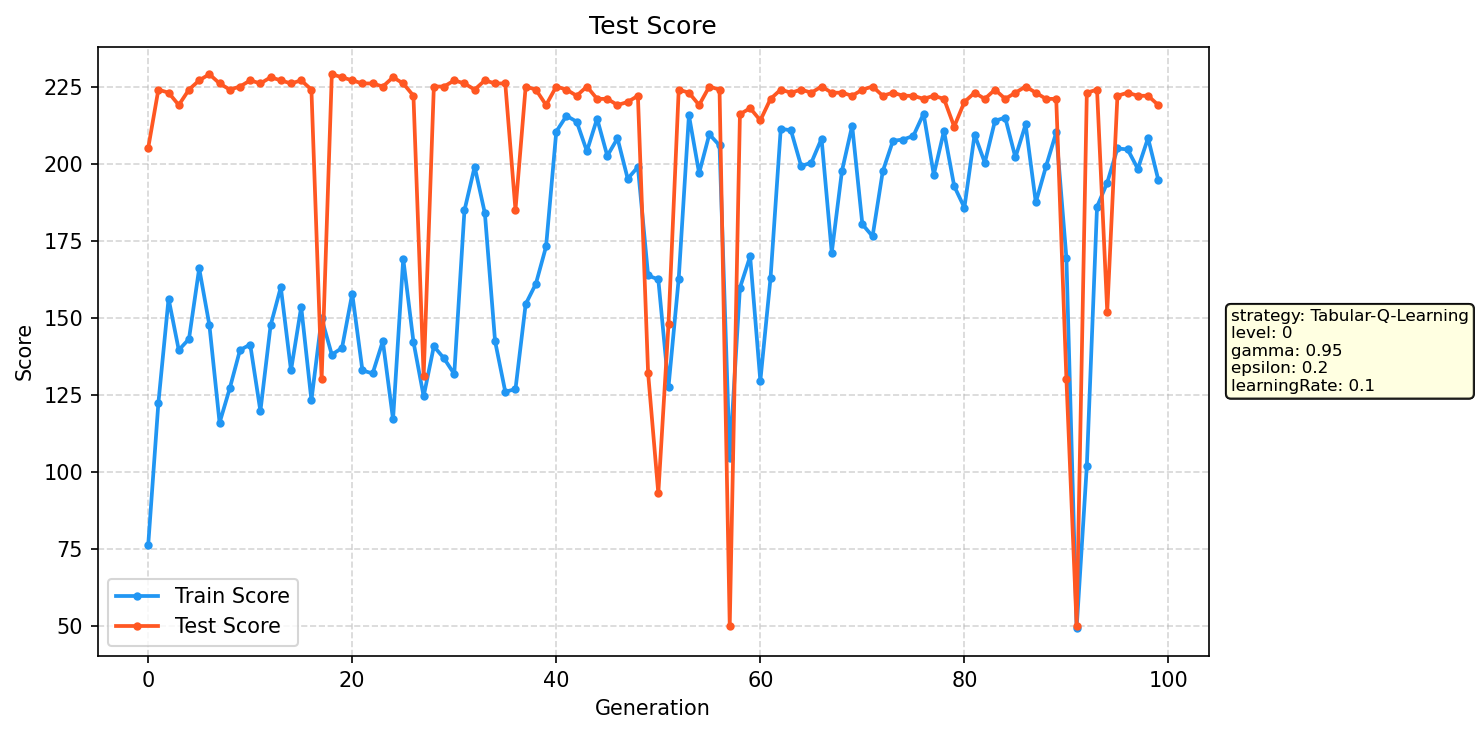
\includegraphics[width=1.2\textwidth]{level0/Tabular-Q-Learning/version1/level0_Tabular-Q-Learning_version1_plot_scores.png}}  
\end{figure}

\subsection{Niveau 1}

\begin{figure}[H]
    \centering
    \makebox[\textwidth][c]{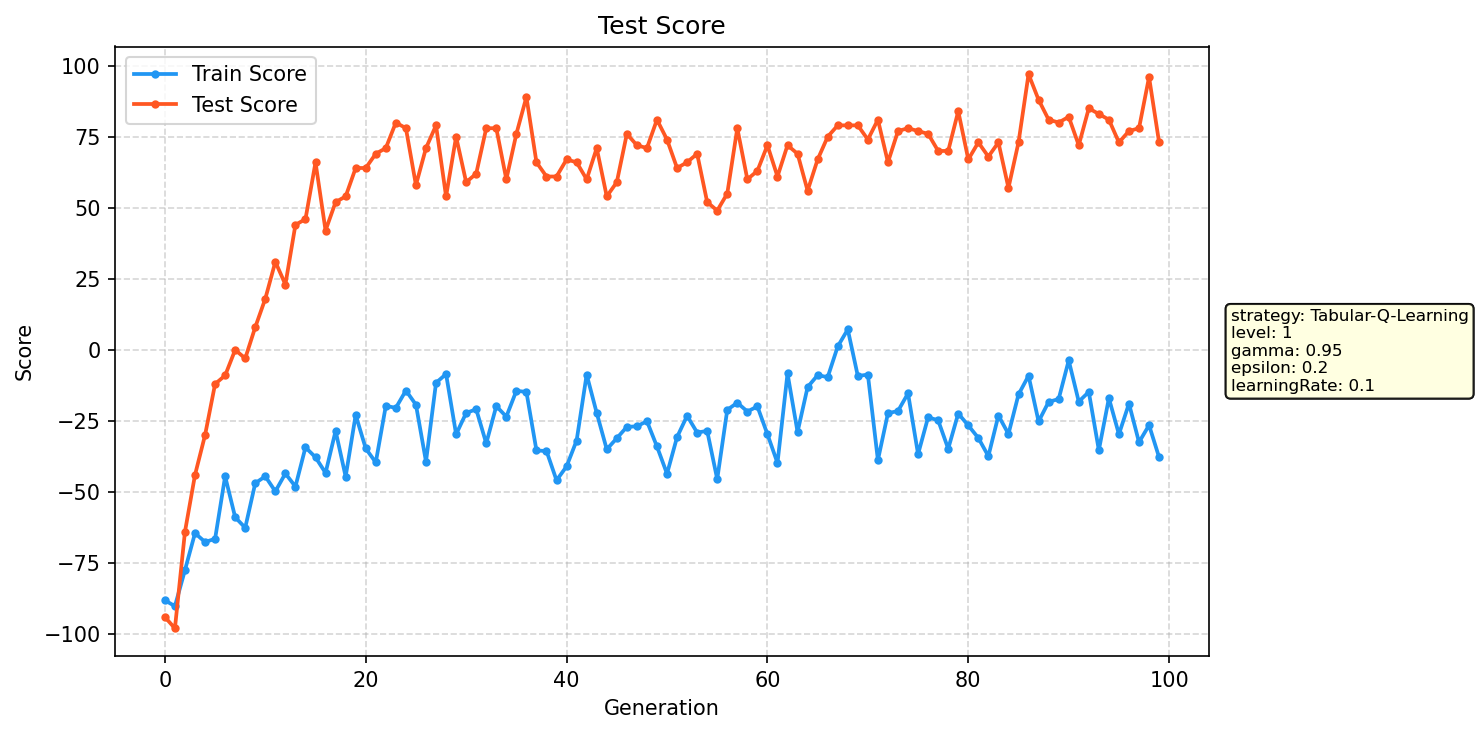
\includegraphics[width=1.2\textwidth]{level1/Tabular-Q-Learning/version1/level1_Tabular-Q-Learning_version1_plot_scores.png}}  
\end{figure}

\subsection{Niveau 2}

\begin{figure}[H]
    \centering
    \makebox[\textwidth][c]{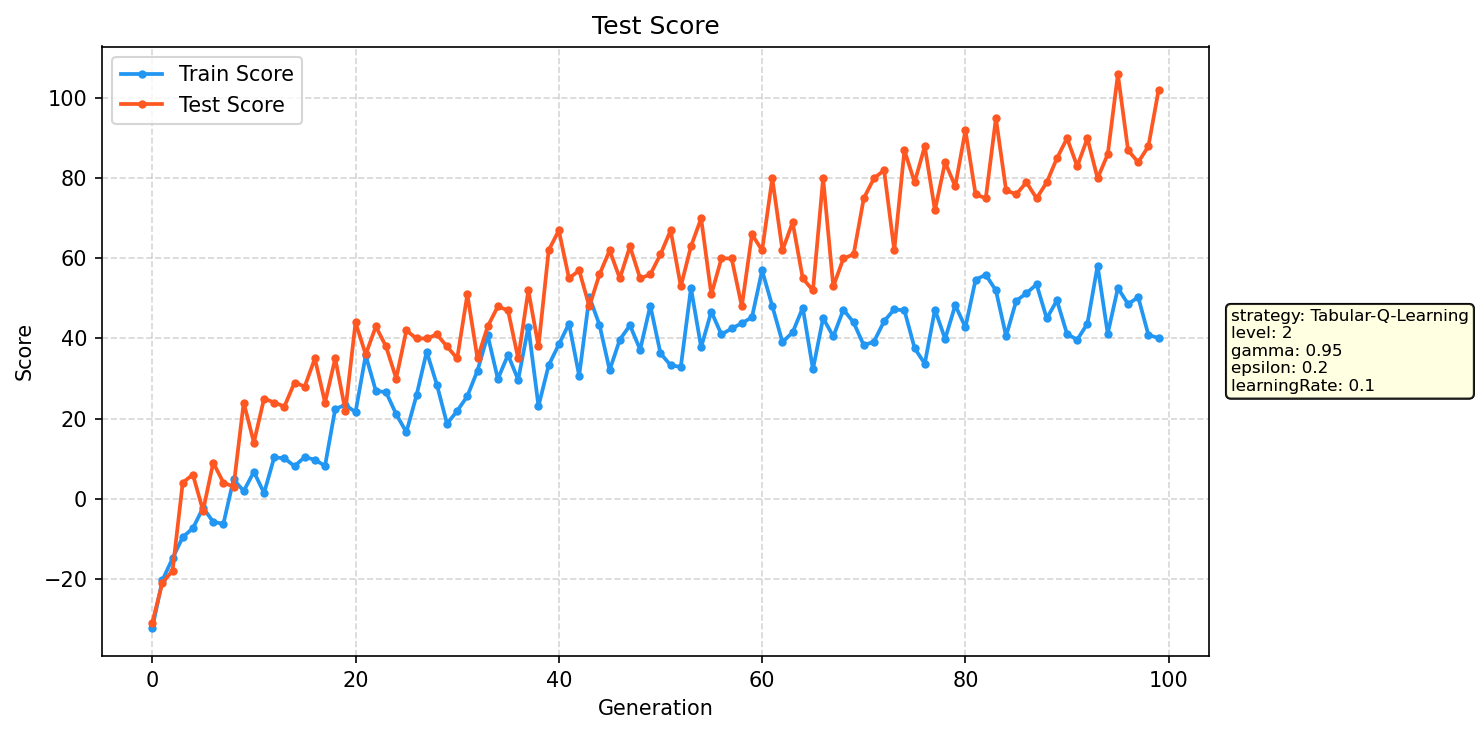
\includegraphics[width=1.2\textwidth]{level2/Tabular-Q-Learning/version1/level2_Tabular-Q-Learning_version1_plot_scores.png}}  
\end{figure}

\subsection{Questions}

\subsubsection{Question 4}

Au fil des générations, l'apprentissage s'améliore, mais il n'est pas stable sur le niveau 0 alors que sur les niveaux 1 et 2, il est plus stable.
La différence de score entre test et apprentissage s'explique par la présence d'exploration dans la phase d'apprentissage (avec le epsilon), 
alors que dans la phase de test, on n'explore plus et on choisit toujours l'action qui maximise la valeur de Q (exploitation).

\subsubsection{Question 5}

Sur le niveau 2, certes le score moyen s'améliore mais il est très faible. En effet, il existe beaucoup d'états et d'actions possibles, ce qui rend l'apprentissage par Tabular Q-Learning plus difficile.
Pour que l'algorithme puisse apprendre l'entiereté des états et actions, il faudrait augmenter considérablement le nombre de générations d'apprentissage, mais cela serait coûteux en temps de calcul et en espace mémoire.
Ainsi le Tabular Q-Learning n'est pas adapté pour ce niveau 2.

\newpage

\section{Exercice 2 : Approximate Q-learning}

\subsection{Niveau 0}

\begin{figure}[H]
    \centering
    \makebox[\textwidth][c]{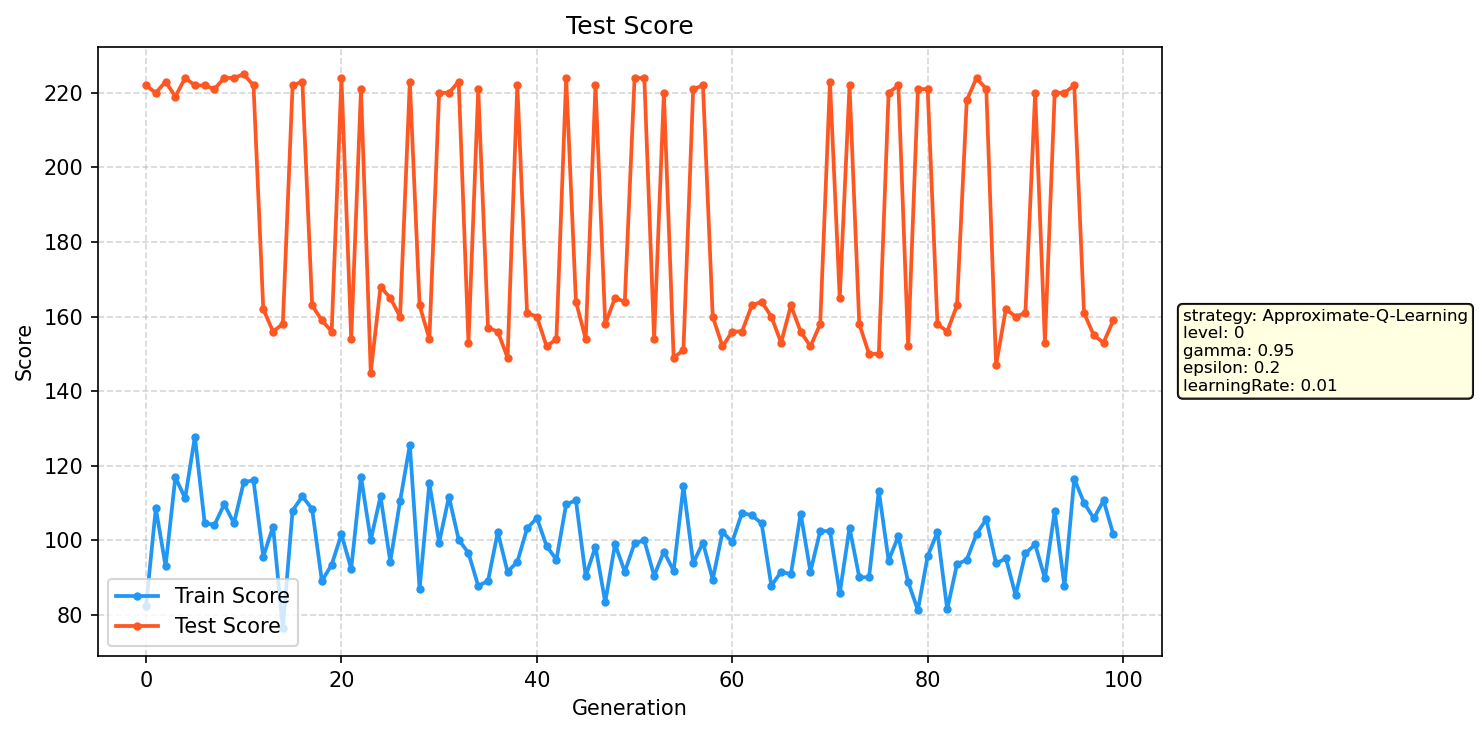
\includegraphics[width=1.2\textwidth]{level0/Approximate-Q-Learning/version1/level0_Approximate-Q-Learning_version1_plot_scores.png}}  
\end{figure}

\subsection{Niveau 1}

\begin{figure}[H]
    \centering
    \makebox[\textwidth][c]{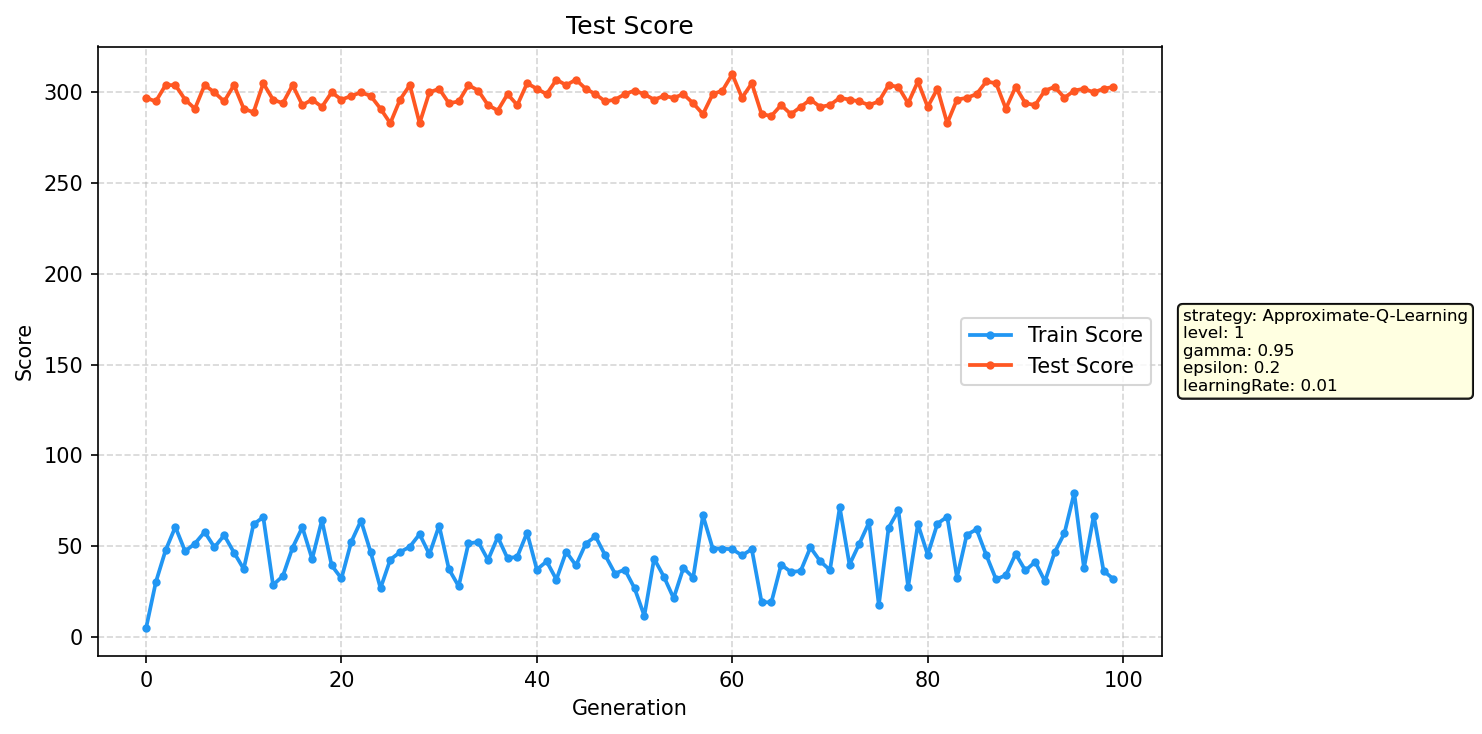
\includegraphics[width=1.2\textwidth]{level1/Approximate-Q-Learning/version1/level1_Approximate-Q-Learning_version1_plot_scores.png}}  
\end{figure}

\subsection{Niveau 2}

\begin{figure}[H]
    \centering
    \makebox[\textwidth][c]{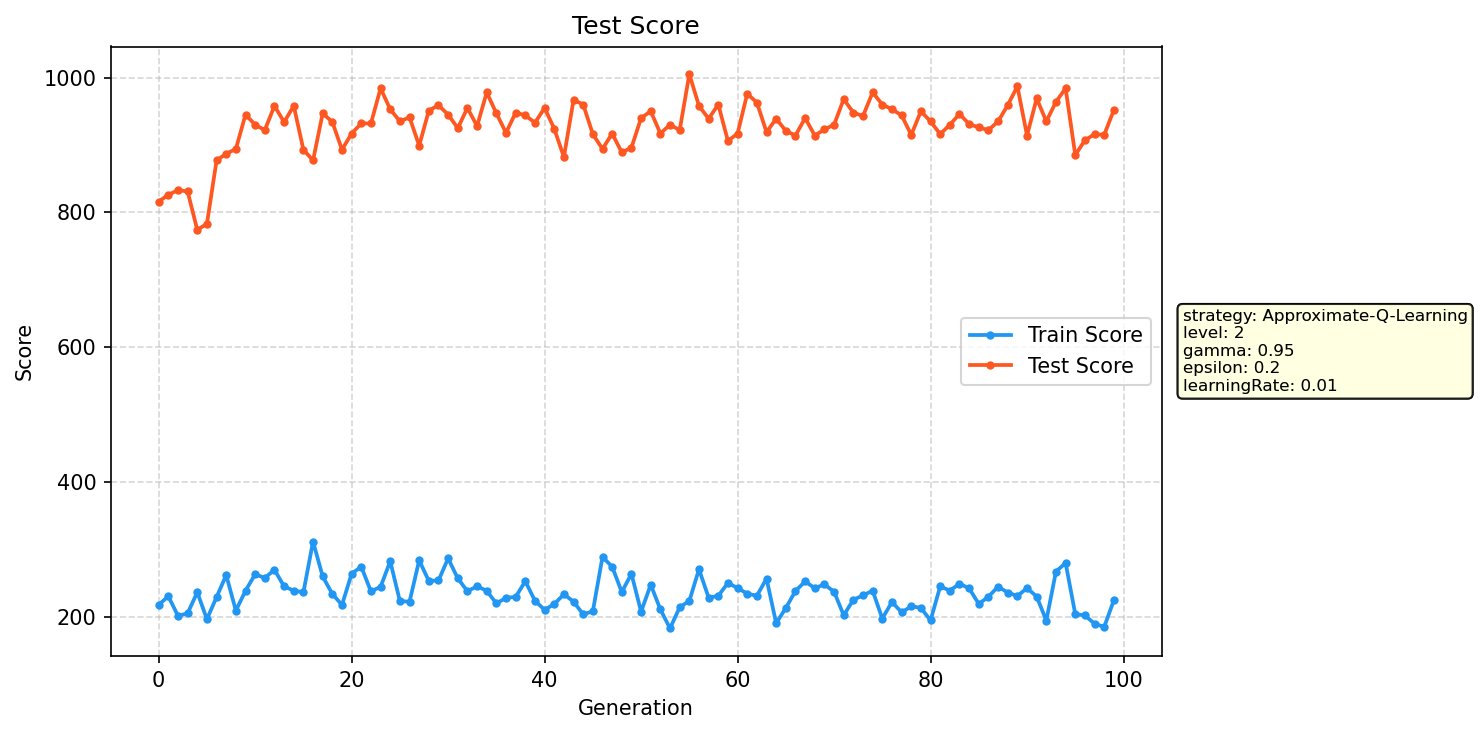
\includegraphics[width=1.2\textwidth]{level2/Approximate-Q-Learning/version1/level2_Approximate-Q-Learning_version1_plot_scores.png}}  
\end{figure}

\subsection{Questions}

\subsubsection{Question 2}

J'ai choisi d'implémenter les features suivantes :

\begin{itemize}
    \item La distance entre le Pacman et la gomme la plus proche.
    \item La distance entre le Pacman et la capsule la plus proche.
    \item La distance entre le Pacman et le fantôme le plus proche ou l'opposé de cette distance si les fantômes sont effrayés.
\end{itemize}
 
J'ai normalisé ces features en divisant 1 par la distance, ce qui permet d'avoir des valeurs plus petites et de mieux gérer les situations où les distances sont grandes.

\subsubsection{Question 3 et 5}

Pour le niveau 0, l'Approximate Q-Learning souffre d'un manque de stabilité. 
Cependant, pour les niveaux 1 et 2, on observe une amélioration rapide du score moyen après quelques générations, ce qui indique que l'agent apprend à mieux jouer, malgré une certaine instabilité.
L'Approximate Q-Learning est plus adapté que le Tabular Q-Learning pour les niveaux 1 et 2, car il peut généraliser à partir d'un nombre limité de features, ce qui lui permet d'apprendre plus efficacement dans des environnements avec un grand nombre d'états et d'actions possibles.
Il pourrait être intéressant d'implémenter d'autres features pour améliorer les performances de l'agent.

\subsubsection{Question 6}

Il y a à minima deux limites importants à cet algorithme. 
Premièrement, il faut spécifier manuellement les features, ce qui peut être difficile et limiter les performances de l'agent si les features choisies ne sont pas pertinentes contrairement au Tabular Q-Learning ou au Deep Q-Learning qui n'ont pas besoin de features manuelles. 
Deuxièmement, l'Approximate Q-Learning suppose que la valeur d'un état est simplement une somme pondérée des features, mais les relations entre features peuvent être bien plus complexes et il ne peut pas les capturer car il est contraint par sa linéarité.

\section{Exercice 3 : Approximate Q-learning with Neural Network}

Non traité.

\section{Exercice 4 : Deep Q-learning}

Non traité.

\end{document}